%!TEX root = ../dokumentation.tex
\chapter{Grundlagen Laserentferungsmessung}\label{chap:grund_lidar}
Um eine Entfernung zu einem Punkt mittels Licht zu bestimmen gibt es verschiedene Möglichkeiten, welche im folgenden Kapitel näher behandelt werden. Ein wichtiger Hinweiß ist zudem, dass im Zusammenhang mit dem Thema \ac{LIDAR} oftmals der Begriff '\acf{ToF}' fällt, dieser beschreibt allerdings nicht immer das direkt damit verbundene Verfahren, sondern allgemein die Entfernungsbestimmung mittels Laufzeit Elektromagnetischer Wellen. Im folgenden Bericht wird mit \ac{ToF} immer das Verfahren der Lichtlaufzeitmessung gemeint.  
\section{Lichtlaufzeitmessung}
\subsection{Grundprinzip}
Das Grundprinzip der Lichtlaufzeitmessung oder auch \acf{ToF} (Abbildung: \ref{tof}), bezieht sich auf die Zeit, welche ein ausgesandter Lichtimpuls benötigt bis er wieder am Sender eintrifft.\\
\begin{figure}[H]
	\centering
	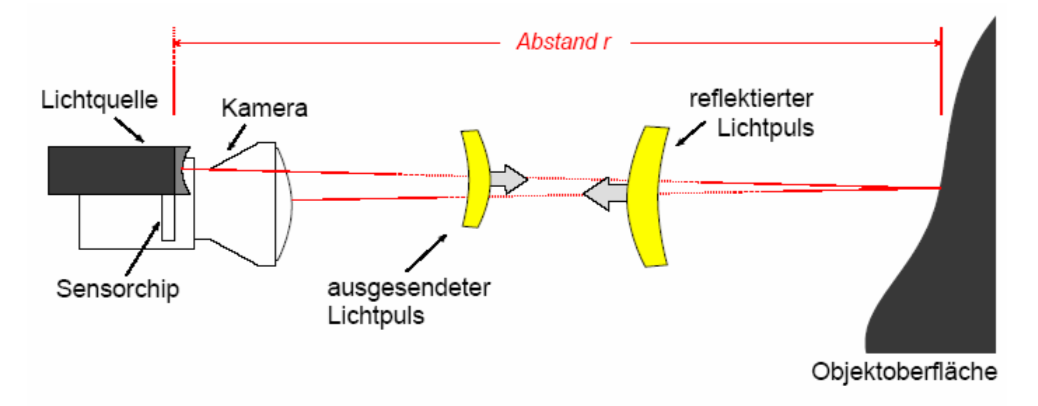
\includegraphics[width=0.75\textwidth]{images/GrundlagenLaserentfernungsmessung/ToF}
	\caption{\ac{ToF} Prinzip \cite{ToF_TUBerlin}}
	\label{tof}
\end{figure}
Dazu wird ein einzelner kurzer Lichtpult von der Lichtquelle ausgesandt, welcher dann von der Oberfläche reflektiert wird und anschließend von einem Sensorchip wieder detektiert werden kann. Über die Zeitdifferenz zwischen Aussenden und Detektieren des Lichtimpulses und die (halbe) Lichtgeschwindigkeit kann anschließend auf die Entfernung des getroffenen Punktes geschlossen werden. \cite{ToF_ST}
\begin{equation}\formelentry{Berechnung der Entfernung mittels Lichtlaufzeit}\label{lichtlaufzeit}
	r = \frac{t_{diff}}{2} \cdot c
\end{equation} 
\begin{flalign*}
	&r = \text{Abstand zum getroffenen Punkt } \left[m \right]&\\
	&t_{diff} = \text{Zeitdifferenz zwischen Aussenden und Detektieren des Lichtpulses}\left[s \right]&\\
	&c = \text{Lichtgeschwindigkeit in Luft}\left[\frac{m}{s} \right]&
\end{flalign*}
Ein großer Vorteil des \ac{ToF} Verfahrens ist, dass durch die Reflexion von Partikeln in der Luft beispielsweise auf die Luftqualität oder die Luftfeuchtigkeit geschlossen werden kann. Dies macht sich am Sensor als vor der größten Reflexion (Oberfläche) auftretende kleine Reflexion bemerkbar.
\subsection{Herausforderungen}\label{subsec:tof_herausvorderungen}
Bei dieser Technologie entstehen allerdings einige Probleme, auf welche im Folgenden eingegangen wird. Generell sind alle Probleme welche bei \ac{ToF} auftreten miteinander verknüpft, bzw. bedingen sich gegenseitig. \\
Das erste Problem welches Auftritt ist, dass nie das gesamte ausgesandte Licht zur Detektion zur Verfügung steht. Durch verschiedene Reflexionsgrade verschiedener Oberflächen und die generelle Streuung des Lichts bei Auftreffen auf eine Oberfläche wir immer nur ein geringer Teil direkt zum Sensor zurückgeworfen. Daher sind hoch empfindliche Sensoren nötig um eine zuverlässige Detektion zu ermöglichen.
\ac{SPAD} sind für die Anwendung in einem \ac{ToF} \ac{LIDAR} System sehr gut geeignet. Vor allem in einer Anordnung zu einem Array, da eine größere Sensorfläche mit gleichbleibender Genauigkeit realisiert werden kann, und somit eine größere Streuung des reflektierten Lichts abgedeckt werden kann. Allerdings ist das Detektieren des zurückgeworfenen Lichts nicht die einzige Herausforderung welche auftritt, denn mit steigender Distanz nimmt die Dämpfung des Lichtimpulses immer weiter ab. 
Eine Lösung dafür könnte sein, eine stärkere Lichtquelle zu verwenden, dies birgt allerdings große Sicherheitsrisiken und ist daher nur begrenzt möglich. Eine zweite Lösung ist, die maximale Messentfernung zu limitieren, allerdings birgt dies ein anderes Problem. Dieses und ein weiteres Problem, welches im Zusammenhang mit der minimalen Messentfernung steht, wird anhand eines Beispiels erläutert.\\
Man nehme an, es existiert ein fiktiver \ac{LIDAR} Sensor mit folgenden Werten:
\begin{itemize}
	\item Minimale Messentfernung $d_{min}=1\:cm$
	\item Maximale Messentfernung $d_{max}=1000\: m$
	\item Maximale Messfrequenz $f_{max}=150\: kHz$ 
\end{itemize}
Formel \ref{lichtlaufzeit} kann umgestellt werden, um die Zeiten zu errechnen, welche das Licht für die minimale und maximale Messentfernung benötigt. 
\begin{equation}\formelentry{Berechnung der minimalen und maximalen Zeit}
	\begin{split}
		t = \frac{r \cdot 2}{c}\\
		t_{min} = \frac{0.01 m \cdot 2}{299,79 \cdot 10^6\: \frac{m}{s}} = 667,13 \cdot 10^{-9}\:s\\
		t_{max} = \frac{1000 m \cdot 2}{299,79 \cdot 10^6\: \frac{m}{s}} = 6,6713 \cdot 10^{-6}\:s\\
	\end{split}
\end{equation} 
\begin{flalign*}
	&r = \text{Abstand zum getroffenen Punkt } \left[m \right]&\\
	&t = \text{Zeitdifferenz zwischen aussenden und detektieren des Lichtpulses}\left[s \right]&\\
	&c = \text{Lichtgeschwindigkeit in Luft}\left[\frac{m}{s} \right]&
\end{flalign*}
Anhand des Beispiels kann man bereits erkennen, dass um die gewünschte minimale Messentfernung zu realisieren eine extrem schnelle Schaltung nötig ist, um das Aussenden und Empfangen innerhalb von $667,13\:ns$ zu detektieren. Die maximale Messentfernung bringt in diesem Fall ein anderes Problem mit sich, welches noch nicht erwähnt wurde. Zwar ist dies nur ein fiktives Beispiel, allerdings muss das Problem trotzdem betrachtet werden. Der Sensor ist mit einer Maximalen Frequenz von $150\:kHz \rightarrow 6,6667\:\mu s$ angegeben, allerdings kann mit dieser Frequenz die maximale Messentfernung nicht erreicht werden, da das Licht länger benötigt um reflektiert zu werden, als die Taktzeit des Sensors ist. \\
Durch dieses Beispiel wurde veranschaulicht, dass verschiedene Faktoren die Grenzen des Sensors festlegen. Die minimale Messentfernung wird dadurch definiert, wie schnell die Schaltung Aussenden und Empfangen detektieren kann. Die maximale Messentfernung wird von der Leistung der Lichtquelle sowie Genauigkeit des Sensors definiert. Die maximale Messfrequenz hängt zusätzlich noch davon ab, wie schnell der Sensor die Daten zur Weiterverarbeitung z.B. an einer \ac{UART} Schnittstelle bereitstellen  kann.

\section{Phasenverschiebung / Phasenmodulation}  \label{sec:phasenverschiebung}
Das Phasenverschiebungsverfahren macht sich zu nutzen, dass bei einer ausgesandten Elektromagnetischen Welle die Phase immer größer wird bei steigender Entfernung. Durch Aussenden verschieden frequentierter Wellen kann dann die Phasenverschiebung der Wellen bestimmt werden und daraus die Entfernung.\cite{phasenverschiebung}\\
\subsection{Grundprinzip}
Das Grundprinzip des Phasenverschiebungsverfahren basiert auf der Interferometrie.\\
Die Interferometrie besagt lediglich, dass die Messergebnisse auf der Interferenz, also der Überlagerung mehrerer Wellen, beruht. Interferenzen treten bei verschiedensten Formen von Wellen auf, nicht nur bei Elektromagnetischen Wellen, sondern auch bei z.B. mechanischen Wellen wie Schall- oder Wasserwellen.\cite{inferometrie}\\
\begin{figure}[H]
	\centering
	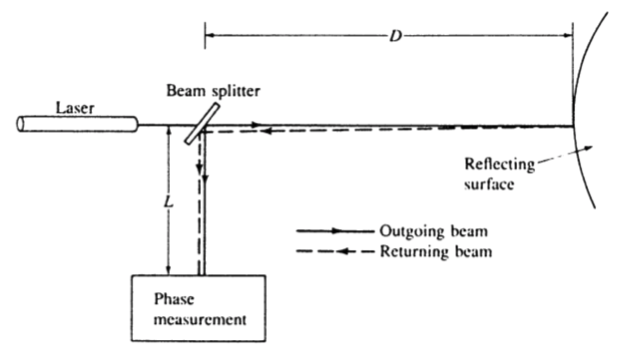
\includegraphics[width=0.75\textwidth]{images/GrundlagenLaserentfernungsmessung/Phasenverschiebung}
	\caption{Versuchsaufbau Phasenverschiebungsentfernungsmessung \cite{lichtabstandsmessung}}
	\label{phasenverschiebung}
\end{figure}
Bei einem Versuchsaufbau nach dem Prinzip in Abbildung \ref{phasenverschiebung}, wird der vom Laser ausgesandte Lichtstrahl zuerst aufgeteilt, damit dieser dann als Referenzwert zur Bestimmung der Phasendifferenz verwendet werden kann. Der zweite Pfad des Lichtstrahls wird sich weiter in Richtung der Oberfläche bewegen, bis dieser schließlich von der Oberfläche reflektiert wird und durch einen Umlenkspiegel ebenfalls zur Bestimmung der Phasendifferenz verwendet wird.\\
Wenn die Distanz $D=0$ ist, kommen die beiden Lichtstrahlen gleichzeitig bei der Phasenbestimmung an. Bei einer Entfernung ungleich 0 ist die zurückgelegte Strecke des Lichtstrahls.
\begin{equation}\formelentry{Zurückgelegte Strecke des Lichtstrahls}
	E = L + 2 \cdot D
\end{equation} 
\begin{flalign*}
	&E = \text{Zurückgelegte Strecke des Lichtstrahls} \left[m \right]&\\
	&L = \text{Abstand zwischen Spiegel und Phasenbestimmung}\left[m \right]&\\
	&D = \text{Abstand zwischen Spiegel und Oberfläche}\left[m \right]&
\end{flalign*} 
Da wie bereits erwähnt die Phase mit steigender Entfernung größer wird kann von dieser Phasenänderung auf die Wellenlänge geschlossen werden. 
\begin{figure}[H]
	\centering
	\includegraphics[width=0.75\textwidth]{images/GrundlagenLaserentfernungsmessung/phase}
	\caption{Phasendifferenz einer Welle \cite{frauenhoferipm}}
	\label{phasendifferenz}
\end{figure}
Die Phase kann als ein Vielfaches der Wellenlänge $\lambda = \frac{c}{f}$ und somit als Entfernung ausgedrückt werden. 
\begin{equation}\formelentry{Zurückgelegte Strecke des Lichtstrahls}\label{streckephase}
	\begin{split}
		\varphi = \frac{4\cdot\pi \cdot D}{\lambda}\\
		D = \frac{c\cdot\varphi}{4\cdot\pi\cdot f_{m}}
	\end{split}
\end{equation} 
\begin{flalign*}
	&D = \text{Abstand zwischen Laser und Oberfläche}\left[m \right]&\\
	&\varphi = \text{Phasendifferenz} \left[^{\circ} \right]&\\
	&\lambda = \text{Wellenlänge}\left[m \right]&\\
	&f_{m} = \text{Modulationsfrequenz} \left[\frac{1}{s} \right]&\\
	&c = \text{Lichtgeschwindigkeit} \left[\frac{m}{s} \right]&
\end{flalign*}
Allerdings bringt die Verwendung nur einer Wellenlänge zur Modulation des Lasers zur Bestimmung der Phasendifferenz einige Probleme mit sich. Zum Einen wird die Gleichung \ref{streckephase} bei jedem Vielfachen $n$ von $360^{\circ}$ die gleiche Lösung ergeben, somit kann man die Distanz nicht eindeutig bestimmen. Zum Anderen ist der Aufbau wie in \ref{phasenverschiebung} nur für wenige Anwendungen geeignet, daher wurde in Abbilding \ref{phasendifferenz} bereits ein anderer besser nutzbarer Aufbau gezeigt. \\
Das Problem der Uneindeutigkeit kann gelöst werden, indem der Lichtstrahl kontinuierlich mit mehreren Signalen mit unterschiedlichen Frequenzen moduliert wird. Anschließend wird für jede der ausgesandten Frequenzen die Phasendifferenz bestimmt. Dies bringt den großen Vorteil, dass durch Überlagerung der Ergebnisse eine Eindeutigkeit festgestellt werden kann und sich die Messgenauigkeit somit deutlich erhöht.\cite{lichtabstandsmessung}\cite{phasenmodulation}\cite{frauenhofer}\\
Einige der Vorteile, welche beim Phasenverschiebungsverfahren bestehen sind, dass die Bauteile um ein Vielfaches langsamer sein können, als beim \ac{ToF} Verfahren. Dies ist darauf zurückzuführen, dass es prinzipiell egal ist bei welchem Nulldurchgang einer Welle die Phase bestimmt wird, da sich nur ein Vielfaches von $360^{\circ}$ zur Phase addiert wird. Durch Verwendung mehrerer Modulationsfrequenzen kann trotzdem eine Eindeutigkeit gewährleistet werden.\\
Dazu kommt auch, dass mit Modulationsfrequenzen im Megahertz Bereich sehr hohe Messgenauigkeiten möglich sind, da diese von der hochsten Modulationsfrequenz abhängt.
\begin{equation}\formelentry{Beispielrechnung Messgenauigkeit}\label{streckephase}
	\lambda = \frac{c}{f_{m}} = \frac{c}{150\cdot 10^{6} Hz} \approx 2\:m
\end{equation} 
\begin{flalign*}
	&\lambda = \text{Wellenlänge}\left[m \right]&\\
	&f_{m} = \text{Modulationsfrequenz} \left[\frac{1}{s} \right]&\\
	&c = \text{Lichtgeschwindigkeit} \left[\frac{m}{s} \right]&
\end{flalign*}
Bei einer Wellenlänge von $2\:nm$ liegt der eindeutige Bereich zwar nur noch bei einem Meter, jedoch lässt sich die Phasendifferenz sehr genau bestimmen und somit ist eine höhere Genauigkeit möglich als besipielsweise bei einer Wellenlänge von $150\: m$.
\subsection{Herausforderungen}
Eine der größten Herausforderungen des Phasenverschiebungsverfahrens sind Störeinflüsse aus der Umwelt. Regen beispielsweise kann sich sehr störend auf die Messergebnisse auswirken. Ebenfalls kann keine zusätzliche Information aus der Reflexion erlangt werden, wie dies beispielsweise beim \ac{ToF} Verfahren möglich ist.\\
Die zum \ac{ToF} Verfahren vergleichsweise wenigen Herausforderungen sind Grund dafür, dass das Phasenverschiebungsverfahren sehr weit verbreitet ist und viele Anwendungen findet.
\section{Triangulation}
Beim Triangulationsverfahren wird sich wie der Name schon vermuten lässt die Trigonometrie zu nutzen gemacht.\\

\subsection{Grundprinzip}
Wenn bei einem Dreieck zwei Punkte, deren Distanz zueinander und der Winkel zum dritten Punkt bekannt ist, dann auch die Position des dritten Punktes bestimmt werden (Abbildung \ref{triangulation}).
\begin{figure}[H]
	\centering
	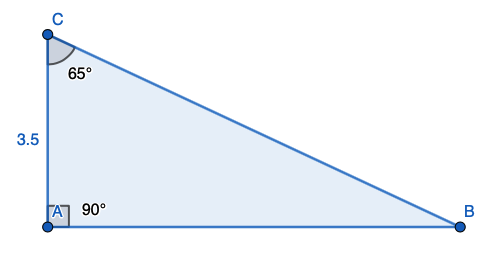
\includegraphics[width=0.75\textwidth]{images/GrundlagenLaserentfernungsmessung/Triangulation}
	\caption{Beispiel Triangulation}
	\label{triangulation}
\end{figure}
Nun kann durch Anwendung bekannter Trigonometrischer Funktionen die Position des dritten Punktes, und damit die Entfernung, bestimmt werden.
\begin{equation}\formelentry{Sinussatz}\label{trigonometrie}
	\frac{c}{sin(\gamma)} = \frac{b}{sin(\beta)} = \frac{a}{sin(\alpha)} 
\end{equation}
\begin{flalign*}
	&a = \text{Stecke BC}\left[m \right]&\\
	&b = \text{Strecke AC} \left[m \right]&\\
	&c = \text{Strecke AB} \left[m \right]&\\
	&\alpha = \text{Winkel an A} \left[^{\circ} \right]&\\
	&\beta = \text{Winkel an B} \left[^{\circ} \right]&\\
	&\gamma = \text{Winkel an C} \left[^{\circ} \right]&
\end{flalign*}
Für das gegebene Beispiel ist dies:
\begin{equation}\formelentry{Beispielrechnung Trigonometrie}\label{bsp_trigonometrie}
	\begin{split}
		\beta = 180^{\circ} - \alpha - \gamma = 25^{\circ}\\
		c = \frac{b\cdot sin(\gamma)}{sin(\beta)} = 7.5\\
		a = \frac{b\cdot sin(\alpha)}{sin(\beta)} = 8.28
	\end{split}
\end{equation}
Da die Winkel bekannt sind, ist nun bekannt, dass der Punkt B an $x = 7.5$ und $y = 0$ liegt. Somit wurde die Entfernung bestimmt.\\
Der Aufbau wie in Abbildung \ref{triangulation} kann auch mit Sender und Empfänger realisiert werden. Dazu wird angenommen, dass in Punkt A ein Sender, also Laser oder \ac{LED} (nur für geringe Anforderungen) positioniert wird. In Punkt C wird ein \ac{PSD} positioniert.\\
Wenn man nun eine Bikonvexe Linse vor das \ac{PSD} positioniert, wird das gesamte einfallende Licht gebündelt und als ein Punkt auf dem \ac{PSD} messbar.
Durch den Abstand des \ac{PSD} zur Linse und die Position des Lichtpunkts auf dem \ac{PSD} lässt sich dann der Winkel des einfallendes Lichts bestimmen.\\
Dieser Winkel kann dann wie beschrieben zur Bestimmung der Entfernung der reflektierenden Oberfläche verwendet werden. \\
Ein sehr großer Vorteil des Triangulationsverfahrens ist, dass es mit sehr preiswerten Bauteilen realisiert werden kann, da wie bereits erwähnt für Anwendungen mit sehr niedrigen Anforderungen eine \ac{LED} als Lichtquelle ausreicht. Ebenfalls sind die Photodioden nicht kompliziert oder teuer, anders als beispielsweise \ac{SPAD} Dioden welche für \ac{ToF} oder Phasenverschiebung Verfahren verwendet werden.\\
Zudem kann durch konstantes Einschalten der Lichtquelle sehr gut eine Geschwindigkeit bestimmt werden, da die \ac{PSD} innerhalb von wenigen Nanosekunden ihren Strom ändern und somit eine sehr schnelle Detektion eines sich bewegenden Objekts möglich ist. \cite{triangulation}\cite{psd}
\subsection{Herausforderungen}
Durch Störeinflüssen wie beispielsweise anderes einfallendes Licht kann die Messung stark beeinflusst werden. Ebenfalls kann es gerade durch die Verwendung von preiswerten Bauteilen zu großen Toleranzen kommen, wodurch die Messergebnisse stark schwanken können. Auch kann ähnlich wie beim Phasenverschiebungsverfahren keine Auskunft über weitere Parameter gegeben werden. 